\documentclass[journal,10pt,twocolumn]{article}
\usepackage{graphicx}
\usepackage[margin=0.5in]{geometry}
\usepackage[cmex10]{amsmath}
\usepackage{array}
\usepackage{booktabs}
\usepackage{listings}
\usepackage{mathtools}
\title{\textbf{Optimization Assignment}}
\author{Panjugala Shashikala}
\date{October 2022}


\providecommand{\norm}[1]{\left\lVert#1\right\rVert}
\providecommand{\abs}[1]{\left\vert#1\right\vert}
\let\vec\mathbf
\newcommand{\myvec}[1]{\ensuremath{\begin{pmatrix}#1\end{pmatrix}}}
\newcommand{\mydet}[1]{\ensuremath{\begin{vmatrix}#1\end{vmatrix}}}
\providecommand{\brak}[1]{\ensuremath{\left(#1\right)}}
\providecommand{\lbrak}[1]{\ensuremath{\left(#1\right.}}
\providecommand{\rbrak}[1]{\ensuremath{\left.#1\right)}}
\providecommand{\sbrak}[1]{\ensuremath{{}\left[#1\right]}}

\begin{document}

\maketitle
\section{Question}
\textbf{The function 
 $f(x)=\int_{-1}^{x}t(e^t-1)(t-1)(t-2)^3(t-3)^5 \,dt$  has a local minimum at x = }

 \section{Solution}
 \textbf{STEP-1}
 The given function \textbf{f(x)} is
 \begin{align}
 f(x)=\int_{-1}^{x}t(e^t-1)(t-1)(t-2)^3(t-3)^5 \,dt 
 \end{align}
Using gradient descent method we can find its minima,
    \begin{align}
        x_{n+1} &= x_n - \alpha \nabla f(x_n) \\
        \implies x_{n+1} &= x_n - \alpha \brak{x(e^x-1)(x-1)(x-2)^3(x-3)^5}
    \end{align}
    
Taking $x_0=0.5,\alpha=0.001$ and precision = 0.00000001, values obtained using python are:
    
    \begin{align}
        \boxed{\text{Minima} = -6967.5283 }\\
        \boxed{\text{Minima Point} = 1.0 }
    \end{align}
    
    
\begin{figure}[h!]
\centering
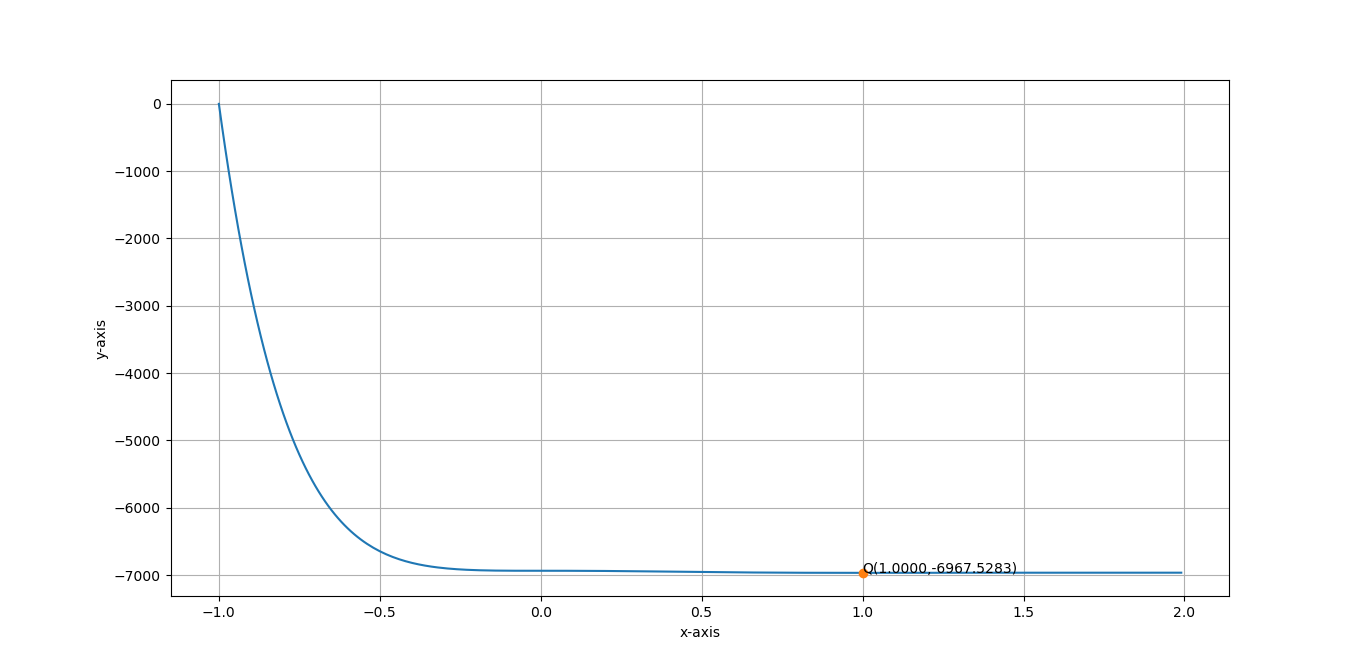
\includegraphics[scale=0.5]{Opt1.png}  \\
\caption{plot of f(x) with minima}
\end{figure}

\end{document}